\documentclass[12pt,fleqn]{article}\usepackage{../common}
\begin{document}
K-Means Kumeleme Metodu

Yapay Ogrenim (Machine Learning) alaninda populer kumeleme
algoritmalarindan biri k-means algoritmasidir. K-means kumelemesinde kac
tane kumenin olmasi gerektigi bastan tanimlanir ($k$ parametresi ile),
algoritma bunu kendisi bulmaz. Metotun geri kalani basit - bir dongu
(iteration) icinde her basamakta:

1) Her nokta icin, eldeki kume merkezleri teker teker kontrol edilir
ve o nokta en yakin olan kumeye atanir

2) Atamalar tamamlandiktan sonra her kume icinde hangi noktalarin
oldugu bilindigi icin her kumedeki noktalarin ortalamasi alinarak yeni
kume merkezi hesaplanir. Eski merkez hesaplari atilir.

3) Basa donulur

Dongu tekrar ilk adima dondugunde, bu sefer yeni kume merkezlerini
kullanilarak, ayni adimlar tekrar yapilacaktir.

Fakat bir problem yok mu? Daha birinci dongu baslamadan kume
merkezlerinin nerede oldugunu nereden bilecegiz? Burada bir
tavuk-yumurta problemi var, kume merkezleri olmadan noktalari
atayamayiz, atama olmadan kume merkezlerini hesaplayamayiz.

Bu probleme pratik bir cozum ilk basta kume merkezlerini (ya da kume
atamalarini) rasgele bir sekilde secmektir. Pratikte bu yontem cok iyi
isliyor. Tabii bu rasgelelik yuzunden K-means'in dogru sonuca
yaklasmasi (convergence) garanti degildir, ama gercek dunya
uygulamalarinda cogunlukla kullanisli kumeler bulunur. Bu potansiyel
problemlerden kacinmak icin k-means pek cok kez isletilebilir (her
seferinde yeni rasgele baslangiclarla yani) ve ayni sonuca ulasilip
ulasilmadigi kontrol edilebilir.

Pek en iyi k nasil bulunur? Burada da yapay ogrenim literaturunde pek
cok yaklasim vardir [1], veriyi pek cok parcaya bolup, farkli k kume
sayisi icin kumeleme yapmak ve capraz saglama (cross-validation)
kullanmak, SVD kullanarak grafige bakmak (bu yazinin sonunda
anlatiliyor), vs.

K-Means EM algoritmasinin bir turevi olarak kabul edilebilir, EM
kumeleri bir Gaussian (ya da Gaussian karisimi) gibi gorur, ve her
basamakta bu dagilimlarin merkezini, hem de kovaryansini
hesaplar. Yani kumenin "sekli" de EM tarafindan saptanir. Ayrica EM
her noktanin tum kumelere olan uyeliklerini "hafif (soft)" olarak
hesaplar (bir olasilik olcutu uzerinden), fakat K-Means icin bu atama
nihai (hard membership). Nokta ya bir kumeye aittir, ya da
degildir.

EM'in belli sartlarda yaklasiksalligi icin matematiksel ispat
var. K-Means akilli tahmin yaparak (heuristic) calisan bir algoritma
olarak biliniyor. Sonuca yaklasmasi bu sebeple garanti degildir, ama
daha once belirttigimiz gibi pratikte faydalidir. Bir suru alternatif
kumeleme yontemi olmasina ragmen hala K-Means'den vazgecilemiyor!
Burada bir etken de K-Means'in cok rahat paralelize edilebilmesi. Bu
konu baska bir yazida islenecek.

Ornek test verisi altta

\begin{minted}[fontsize=\footnotesize]{python}
import pandas as pd
data = pd.read_csv("synthetic.txt",names=['a','b'],sep="   ")
print data.shape
data = np.array(data)
\end{minted}

\begin{verbatim}
(3000, 2)
\end{verbatim}

\begin{minted}[fontsize=\footnotesize]{python}
plt.scatter(data[:,0],data[:,1])
plt.savefig('kmeans_1.png')
\end{minted}

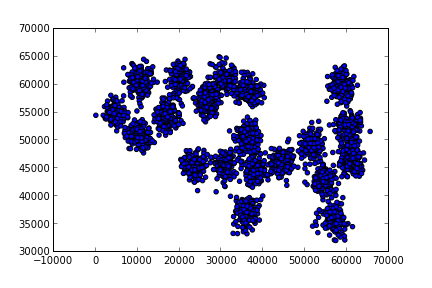
\includegraphics[height=6cm]{kmeans_1.png}
\begin{minted}[fontsize=\footnotesize]{python}
def euc_to_clusters(x,y):
    return np.sqrt(np.sum((x-y)**2, axis=1))

class KMeans():
    def __init__(self,n_clusters,n_iter=10):
        self.k = n_clusters
        self.iter = n_iter
    def fit(self,X):
        # her veri noktasi icin rasgele kume merkezi ata
        labels = [random.randint(0,self.k-1) for i in range(X.shape[0])]
        self.labels_ = np.array(labels)
        self.centers_ = np.zeros((self.k,X.shape[1]))
        for i in range(self.iter):
            # yeni kume merkezleri uret
            for j in range(self.k):
                # eger kume j icinde hic nokta yoksa, ortalama (mean)
                # hesabi yapma, cunku o zaman nan degeri geliyor, ve
                # hesabin geri kalani bozuluyor.
                if len(X[self.labels_ == j]) == 0: continue
                center = np.mean(X[self.labels_ == j],axis=0)
                self.centers_[j,:] = center
            # her nokta icin kume merkezlerine gore kume atamasi yap
            self.labels_ = []
            for point in X:
                c = np.argmin(euc_to_clusters(self.centers_, point))
                self.labels_.append(int(c))

            self.labels_ = np.array(self.labels_)
\end{minted}

\begin{minted}[fontsize=\footnotesize]{python}
cf = KMeans(k=5,iter=20)
cf.fit(data)
print cf.labels_
\end{minted}

\begin{verbatim}
[3 3 3 ..., 2 2 2]
\end{verbatim}

Ustteki sonucun icinde iki ana vektor var, bu vektorlerden birincisi icinde
2,0, gibi sayilar goruluyor, bu sayilar her noktaya tekabul eden kume
atamalari.  Ikinci vektor icinde iki boyutlu $k$ tane vektor var, bu
vektorler de her kumenin merkez noktasi. Merkez noktalarini ham veri
uzerinde grafiklersek (kirmizi noktalar)

\begin{minted}[fontsize=\footnotesize]{python}
plt.scatter(data[:,0],data[:,1])
plt.hold(True)
plt.ylim([30000,70000])
for x in cf.centers_: plt.plot(x[0],x[1],'rd')
plt.savefig('kmeans_2.png')
\end{minted}

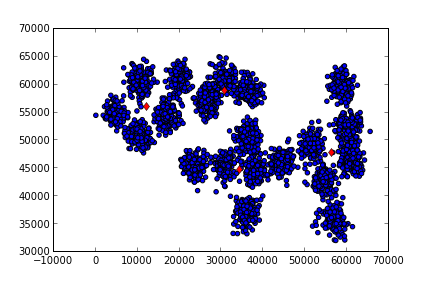
\includegraphics[height=6cm]{kmeans_2.png}

Goruldugu gibi 5 tane kume icin ustteki merkezler bulundu. Fena
degil. Eger 10 dersek

\begin{minted}[fontsize=\footnotesize]{python}
cf = KMeans(k=10,iter=30)
cf.fit(data)
plt.scatter(data[:,0],data[:,1])
plt.ylim([30000,70000])
plt.hold(True)
for x in cf.centers_: plt.plot(x[0],x[1],'rd')
plt.savefig('kmeans_3.png')
\end{minted}

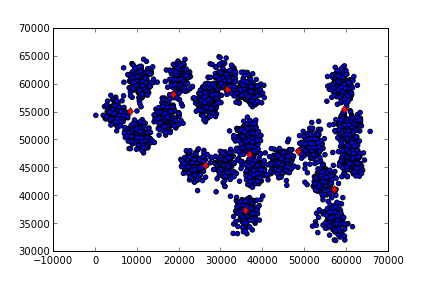
\includegraphics[height=6cm]{kmeans_3.png}

Kategorik ve Numerik Iceren Karisik Veriler

Bazen verimiz hem kategorik hem de numerik degerler iceriyor olabilir,
KMeans yeni kume merkezlerini hesaplarken ortalama operasyonu
kullandigi icin sadece numerik veriler uzerinde calisabilir (kategorik
verilerin nasil ortalamasini alalim ki?). Bu durumda ne yapacagiz?

Bir secenek su olabilir, kategorik her kolonu her degisik degeri bir
yeni kolona tekabul edecek sekilde saga dogru acariz, ve o degerin
yeni kolonuna 1 degeri digerlerine 0 degeri veririz. Bu kodlamaya
1-in-q kodlamasi, 1-in-n kodlamasi, ya da Ingilizce one-hot encoding
ismi veriliyor.

Ornek olarak UCI veri bankasindan Avustralya Kredi Verisine bakalim:

\begin{minted}[fontsize=\footnotesize]{python}
import pandas as pd
df = pd.read_csv("crx.csv")
print df[:2]
\end{minted}

\begin{verbatim}
  A1     A2    A3 A4 A5 A6 A7    A8 A9 A10  A11 A12 A13    A14  A15 A16
0  b  30.83  0.00  u  g  w  v  1.25  t   t    1   f   g  00202    0   +
1  a  58.67  4.46  u  g  q  h  3.04  t   t    6   f   g  00043  560   +
\end{verbatim}

Bu veride A1, A2, gibi kolon isimleri var, kategorik olanlarda 'g','w' gibi
degerler goruluyor. Bu kolonlari degistirmek icin

\begin{minted}[fontsize=\footnotesize]{python}
from sklearn.feature_extraction import DictVectorizer
def one_hot_dataframe(data, cols):
    vec = DictVectorizer()
    mkdict = lambda row: dict((col, row[col]) for col in cols)
    vecData = pd.DataFrame(vec.fit_transform(data[cols].to_dict(outtype='records')).toarray())
    vecData.columns = vec.get_feature_names()
    vecData.index = data.index
    data = data.drop(cols, axis=1)
    data = data.join(vecData)
    return data

df2 = one_hot_dataframe(df,['A1','A4','A5','A6','A7','A9','A10','A12','A13'])
print df2.ix[0]
\end{minted}

\begin{verbatim}
A2       30.83
A3           0
A8        1.25
A11          1
A14      00202
A15          0
A16          +
A10=f        0
A10=t        1
A12=f        1
A12=t        0
A13=g        1
A13=p        0
A13=s        0
A1=?         0
A1=a         0
A1=b         1
A4=?         0
A4=l         0
A4=u         1
A4=y         0
A5=?         0
A5=g         1
A5=gg        0
A5=p         0
A6=?         0
A6=aa        0
A6=c         0
A6=cc        0
A6=d         0
A6=e         0
A6=ff        0
A6=i         0
A6=j         0
A6=k         0
A6=m         0
A6=q         0
A6=r         0
A6=w         1
A6=x         0
A7=?         0
A7=bb        0
A7=dd        0
A7=ff        0
A7=h         0
A7=j         0
A7=n         0
A7=o         0
A7=v         1
A7=z         0
A9=f         0
A9=t         1
Name: 0, Length: 52, dtype: object
\end{verbatim}

Islem sonucunda A12=f mesela icin 1 verilmis, ama A12=t (ve diger her
mumkun deger icin yani) 0 degeri verilmis (sadece bu tek satir
icin). Boylece kategorik veriyi sayisal hale cevirmis olduk.

Fakat isimiz bitti mi? Hayir. Simdi KMeans bu tur veriyle acaba duzgun
calisir miydi onu kendimize soralim. Icinde pek cok 0, bazen 1 iceren 
veri satirlari arasinda uzaklik hesabi yapmak ise yarar mi?

Yapay Ogrenim literaturunde bu tur veriler uzerinde kosinus benzerligi
(cosine similarity) kullanmak daha yaygindir. Bu konuyu {\em SVD, Toplu
  Tavsiye} yazisinda daha iyi gorebilirsiniz. Kosinus benzerligi bize 0 ile
1 arasinda bir deger dondurur. Benzerligi uzakliga cevirmek icin basit bir
sekilde 1-benzerlik formulunu kullanabiliriz. O zaman soyle bir cozum
kullanabilir: normal numerik degerler icin Oklitsel, kategorik 1-hot
kodlanmis kolonlar icin Kosinus uzakligi kullanilir, bu uzakliklar bazi
agirliklar uzerinden birlestirilir, ve KMeans bu uzaklik ile is
yapar. Teknik olarak imkansiz degil; KMeans merkez bulmak icin ortalama
alir ve Kosinus uzakliginin verdigi aradaki aci, ortalama alma islemi ile
uyumludur. Yani icinde hem Oklitsel hem 1-hot kodlanmis verilerin oldugu
vektorlerin ortalamasini alabiliriz, demek ki KMeans isleyebilir.

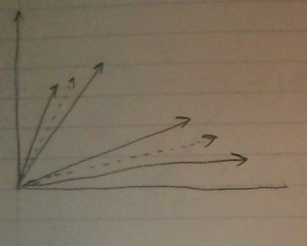
\includegraphics[height=4cm]{kmeans_5.jpg}

Problem sudur, iki uzakligi birlestiren agirliklar ne olmalidir?  Bu
yontemi denedigimizde bu agirliklarin ne secildiginin cok onemli oldugunu
farkettik, ve kumeleme gibi izlenmeyen (unsupervised) bir yontemde bu
hiperparametreleri deneme / yanilma yontemi ile bulma sansimiz yoktur.

Bu durumda kullanilabilecek bir yontem sudur: SVD kullanarak tum matrisi
azaltmak ve onun uzerinde pur Oklitsel uzakliklar kullanmak. Numerik ve
kategorik karisik verileri iceren verileri kumelemek icin tavsiye edilen
yontem sudur:

1) Kategorik veriler uzerinde 1-hot kodlama yap. 

2) Once kolonlari sonra satirlari normalize et.

3) Tum matris uzerinde cok kucuk olmayan bir $k$ ile SVD al (mesela alttaki
veri seti icin once 10)

4) $S$ vektorune bak, ortalamadan buyuk olan kac tane hucre oldugunu gor.

5) Bu sayi yeni $k$ degerimiz olacak, SVD'yi tekrar bu $k$ ile islet. 

6) Elde edilen $U$ uzerinde kumeleme yap,

\begin{minted}[fontsize=\footnotesize]{python}
from sklearn.preprocessing import normalize
import scipy.sparse.linalg as slin
import scipy.linalg as lin
import pandas as pd

df = pd.read_csv("crx.csv",sep=',',na_values=['?'])
df = df.dropna()

df['A16'] = df['A16'].str.replace('+','1')
df['A16'] = df['A16'].str.replace('-','0')
df['A16'] = df['A16'].astype(int)

df2 = one_hot_dataframe(df,['A1','A4','A5','A6','A7','A9','A10','A12','A13'])
df2 = df2.drop('A16',axis=1)
df2 = np.array(df2)
df3 = df2.copy()
df3 = normalize(df3, norm='l2', axis=0)
df3 = normalize(df3, norm='l2', axis=1)

u,s,v=slin.svds(df3,k=10)
print s
\end{minted}

\begin{verbatim}
[  4.45826083   4.49654025   4.68382638   4.93391665   4.98604314
   5.153349     5.63521289   5.70490968   6.68558115  14.81145675]
\end{verbatim}

Bakiyoruz, averajdan yuksek olan en buyuk sadece iki kolon var. SVD
literaturunde bu kolonlarin matrisin ``enerjisini'' icerdigi soylenir,
hakikaten eger SVD ayristirma sonrasi bu ilk kolona bu kadar onem verdiyse,
onlar onemli, ``enerjiyi iceriyor'' olmalidirlar. Simdi SVD'yi $k=2$ ile
tekrar isletiyoruz,

\begin{minted}[fontsize=\footnotesize]{python}
u,s,v=slin.svds(df3,k=2)
print s
\end{minted}

\begin{verbatim}
[  6.68558115  14.81145675]
\end{verbatim}

Simdi $U$ uzerinde kumeleme yapacagiz, ve kontrol icin kenara koydugumuz
bilinen etiketler uzerinden kumeleme basarimizi olcecegiz. Avustralya Kredi
Verisi aslinda izlenen (supervised) algoritmalar icin kullanilir, ama biz
onu izlenmeyen kumeleme problemi icin kullandik, bilinen etiketleri veri
icinden cikartip bir kenara koyuyoruz, ve sonra kumeleme tahmini yaparak bu
etiketlerle olan uyumu olcuyoruz. 

\begin{minted}[fontsize=\footnotesize]{python}
clf = KMeans(n_clusters=2)
clf.fit(u)
labels_true = np.array(df['A16'])
labels_pred = clf.labels_
match = np.sum((labels_true == labels_pred).astype(int))
print float(match)/len(df), 1-float(match)/len(df)
\end{minted}

\begin{verbatim}
0.217457886677 0.782542113323
\end{verbatim}

Basari yuzde \%78. Cok iyi. Ustteki ornek kume sayisinin (dikkat SVD
$k$'sinden farkli) bilindigini farz etti. Kume sayisinin bilinmedigi
durumlarda bile isleyen bir kumeleme algoritmasini baska bir yazida
gorecegiz. 

Bazi ek notlar

[1] \url{http://en.wikipedia.org/wiki/Determining_the_number_of_clusters_in_a_data_set}

[2] \url{nbviewer.ipython.org/url/cbcb.umd.edu/~hcorrada/PML/src/kmeans.ipynb}

[3] \url{https://archive.ics.uci.edu/ml/datasets/Statlog+%28Australian+Credit+Approval%29}
\end{document}
